%
% Tesi D.S.I. - modello preso da
% Stanford University PhD thesis style -- modifications to the report style
%
%%%%%%%%%%%%%%%%%%%%%%%%%%%%%%%%%%%%%%%%%%%%%%%%%%%%%%%%%%%%%%%%%%%%%%%%%%%
%                                                                         %
%			TESI DOTTORATO                                                   %
%			______________                                                   %
%                                                                         %
%			AUTORE: Elena Pagani                                             %
%                                                                         %
%			Ultima revisione: 7.X.1998                                       %
%           correzioni atrent                                             %
%%%%%%%%%%%%%%%%%%%%%%%%%%%%%%%%%%%%%%%%%%%%%%%%%%%%%%%%%%%%%%%%%%%%%%%%%%%
%
%
\documentclass[a4paper,12pt]{report}
%    \renewcommand{\baselinestretch}{1.6}      % interline spacing
%
% \includeonly{}
%
%			PREAMBOLO
%
\usepackage[a4paper]{geometry}
\usepackage{amssymb,amsmath,amsthm}
\usepackage{graphicx}
\usepackage{url}
\usepackage{hyperref}
\usepackage{epsfig}
\usepackage[italian]{babel}
\usepackage{setspace}
\usepackage{tesi}

% Aggiunti da me
\hypersetup{hidelinks}
\usepackage{subcaption}
\usepackage{float}


% per le accentate
\usepackage[utf8]{inputenc}
%
\newtheorem{myteor}{Teorema}[section]
%
\newenvironment{teor}{\begin{myteor}\sl}{\end{myteor}}
%
%
%			TITOLO
%
\begin{document}
\title{Tecniche di machine learning per la classificazione di reperti archeologici}
\author{Pietro Scuttari}
\dept{Corso di Laurea in informatica} 
\anno{2020-2021}
\matricola{922822}
\relatore{Prof.ssa Anna Maria Zanaboni}
\correlatore{Prof. Dario Malchiodi}
%
%        \submitdate{month year in which submitted to GPO}
%		- date LaTeX'd if omitted
%	\copyrightyear{year degree conferred (next year if submitted in Dec.)}
%		- year LaTeX'd (or next year, in December) if omitted
%	\copyrighttrue or \copyrightfalse
%		- produce or don't produce a copyright page (false by default)
%	\figurespagetrue or \figurespagefalse
%		- produce or don't produce a List of Figures page
%		  (false by default)
%	\tablespagetrue or \tablespagefalse
%		- produce or don't produce a List of Tables page
%		  (false by default)
% 
%			DEDICA
%
\beforepreface
% \prefacesection{}
% 		{\hfill \Large {\sl dedicato a \dots}}
% 
%			PREFAZIONE
%
\prefacesection{Prefazione}
\section{Descrizione del problema}
L'obbiettivo di questo progetto è riuscire a risalire all'origine geografica di
alcuni reperti archeologici ritrovati nel sito della necropoli di cerveteri
utilizzando tecniche di machine learning. Per ogni reperto archeologico sono
state eseguite delle analisi di composizione producendo così un database su cui
poter eseguire i diversi algoritmi utilizzati lavorando principalmente su un
sottoinsieme di questi reperti di cui è nota la provenienza per poi applicare i
modelli generati al database completo.


%
%
%			ORGANIZZAZIONE
\section{Organizzazione della tesi}
\label{organizzazione}
La tesi \`e organizzata come segue:
\begin{itemize}
	\item Nel capitolo 1 viene introdotto il progetto introducendo i concetti
	principali e gli algoritmi utilizzati.

	\item Nel capitolo 2 

\end{itemize}
%
%			RINGRAZIAMENTI
%
\prefacesection{Ringraziamenti}
asdjhgftry.
\afterpreface
% 
% 
%			CAPITOLO 1: Introduzione
\chapter{Algoritmi di machine learning e di classificazione}
\label{cap1}

\section{Che cos'è il machine learning}
Machine learning è un nome che include una varietà di algoritmi che, al
contrario di algoritmi tradizionali, non specificano passo per passo come
risolvere un certo problema ma autonomamente creano un modello del problema, in
un processo detto allenamento, a partire da alcune istanze di questo. Otteniamo
così un un modello ovvero una rappresentazione matematica semplificata del
problema originale che usiamo per approssimare una soluzione per ogni istanza
possibile del problema. 

È quindi necessario avere una buona quantità di istanze ognuna composta da più
valori, detti caratteristiche, che vengono tipicamente divise in due parti:
l'insieme di training e l'insieme di di test. Il primo viene usato per
l'allenamento del modello e il secondo per valutare le sue prestazioni, è
importante che questi rimangano separati altrimenti il modello sarebbe
facilitato da aver gia visto i dati durante l'allenamento e non potremmo
valutare la prestazioni reali. 

Esistono due principali sottoinsiemi di algoritmi, quelli detti ad apprendimento
supervisionato e quelli a apprendimento non supervisionato. Nel primo caso il
training set è etichettato ovvero per ogni istanza è specificata la soluzione,
detta etichetta, corrispondente, al contrario questa informazione non è presente
per l'apprendimento non supervisionato. Il primo caso è tipicamente più semplice
data l'informazione ulteriore disponibile e è anche quello principalmente
utilizzato in questo progetto.

\section{Cosa sono i problemi di classificazione}

I problemi di classificazione consistono nel produrre un algoritmo, detto
classificatore, in grado associare a un istanza di input una o più categorie,
come ad esempio una mail a "spam" o "non spam". Questo tipo di problema si presta
molto alle tecniche di machine learning infatti spesso è difficile programmare
manualmente stretti criteri per la classificazione ma è possibile lasciare al
calcolatore questo compito fornendo solo una serie di esempi corretti da cui
possa imparare.

\section{Reti neurali}

Le reti neurali sono una famiglia di modelli ispirati alle reti neuronali
biologiche, sono composti da una serie di neuroni collegati fra loro. Questi
neuroni in realtà non sono altro che una semplice funzione che moltiplica ogni
input $o_i$ per un certo peso $w_i$, i risultati vengono sommati e usati come
argomento di una funzione di attivazione $f$ che produce l'output del neurone:

$$
f(\sum_i o_i w_i)
$$

Spesso è utilizzata una funzione di attivazione che produce risultati compresi
tra 0 e 1 in modo da uniformare gli input del neurone successivo, questo non è
sempre il caso specialmente nell'ultimo strato di neuroni.

Il modo in cui i neuroni sono collegati è detto topologia e nel caso utilizzato
in questo progetto prende il nome di percettrone multistrato. In questa
topologia i neuroni sono organizzati in diversi collegati fra loro in modo che
l'output di ogni strato funge da input per il successivo. Il primo strato è
detto strato di input nel quale abbiamo tanti neuroni quante le caratteristiche
dei dati in ingresso al modello, ognuno di essi elabora una caratteristica
secondo la propria funzione e invia l'output a ogni neurone dello strato
successivo. In seguito abbiamo una serie di strati detti nascosti in cui a ogni
livello i neuroni ricevono l'output di tutti i neuroni nel livello precedente e
inviano il loro risultato a tutti i neuroni del livello successivo. L'ultimo
livello è quello di output in cui i neuroni ricevono l'output dall'ultimo layer
nascosto e restituiscono la soluzione. La dimensione del livello di output è
determinata dalla soluzione desiderata, ad esempio in un problema di
classificazione avremmo tanti neuroni in uscita quante categorie possibili per
la classificazione.

\begin{figure}[h]
	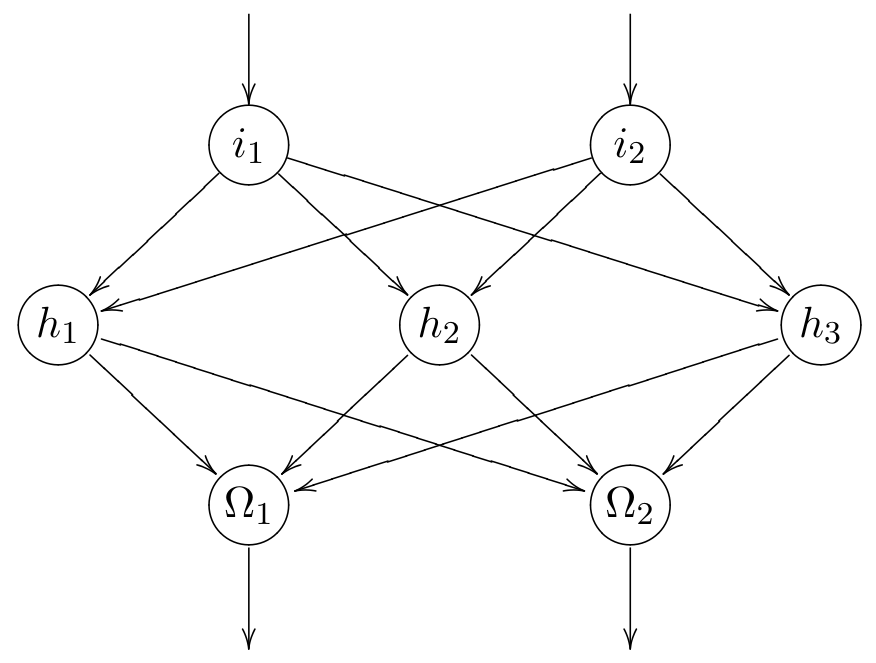
\includegraphics[width = 0.9\textwidth]{Immagini/MLP diagramma.png}
	\captionof{figure}{Semplice rappresentazione di un percettrone multistrato con
	due neuroni di input, tre in un singolo strato nascosto e due in output}
\end{figure}
\newpage

I parametri delle funzioni dei neuroni sono inizializzati con dei valori casuali
e vengono perfezionati durante l'apprendimento il quale, nel nostro caso, sarà
supervisionato: a ogni step si confronta l'output del network con l'etichetta
del dato correggendo poi i valori dei parametri dei neuroni per far avvicinare
la risposta della rete a quella corretta. Il processo viene ripetuto
iterativamente fino a che viene raggiunto un criterio di arresto come un certo
numero di iterazioni, una soglia sull'errore o una soglia sul rateo di
miglioramento. 

All'utente viene lasciato il controllo di quelli che vengono detti iperparametri
ovvero i parametri che controllano il funzionamento della rete neurale e che non
vengono modificati durante l'apprendimento. Alcuni esempi sono la topologia del
network neurale, la funzione di attivazione, la dimensione del passo di
apprendimento eccetera.

%Cost function
%Gradiente
%Backprop 

\section{K-nearest neighbors}

K-nearest neighbors è uno dei modelli più semplici tra quelli usati: invece che
creare un modello interno del problema semplicemente memorizza i dati di
training, ovvero quelli usati durante allenamento, e per classificare una nuova
istanza calcola quali sono i $K$ valori memorizzati più vicini e restituisce
l'etichetta più frequente tra questi.

Uno dei possibili problemi è la poca uniformità dei dati: se i valori più vicini
selezionati sono molto distanti dal punto che stiamo cercando di classificare
potrebbero non essere rilevanti per la classificazione, per ovviare a questo
problema è possibile pesare il calcolo per l'etichetta con la distanza dei punti
dando quindi meno importanza ai punti più distanti. Un importante iperparametro
di cui abbiamo controllo è $K$ ovvero il numero di dati di training da
considerare per calcolare l'etichetta più probabile. La scelta corretta dipende
dal nostro dataset: in generale un valore maggiore di $K$ sarà utile per
superare il rumore statistico dei nostri dati ma produrrà una distinzione meno
netta tra le categorie.

\newpage %La new page serve a posizionare correttamente le immagini successive


\section{Macchine a vettori di supporto}

L'obbiettivo di una macchina a vettori di supporto (SVM) è trovare un iperpiano
che separi i dati di training nelle corrette categorie cercando di massimizzare
il margine, ovvero la distanza tra l'iperpiano e i dati più vicini di ogni
categoria. Fatto questo per classificare un nuovo dato basterà vedere da che
parte dell'iperpiano si trova.

\begin{figure}[h]
	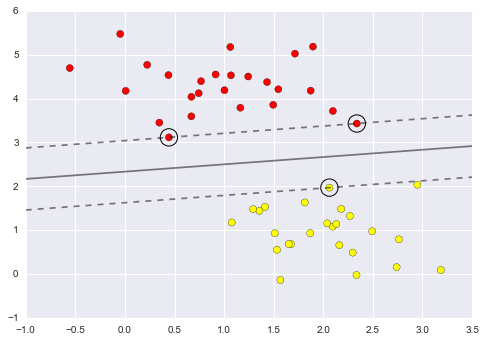
\includegraphics[width =0.9\textwidth]{Immagini/SVM margine.png}
	\caption{Esempio di iperpiano con i limiti del margine evidenziati \cite{Data science handbook}} 
	
\end{figure}

qè necessario trasformare i dati in uno spazio di dimensioni superiori secondo
una funzione di kernel che ci permetta poi di tracciare l'iperpiano. 

\begin{figure}[!h]
	\caption{Esempio dati scalati con funzione kenrel}
	\begin{subfigure}{0.5\textwidth}
		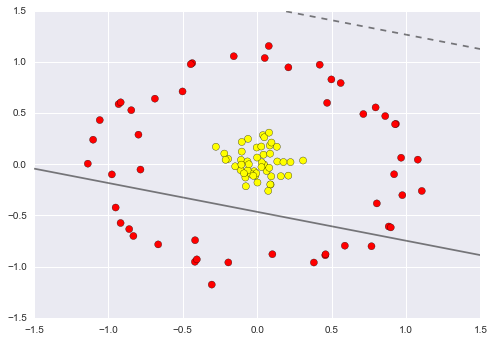
\includegraphics[width=0.9\linewidth]{Immagini/SVm non lineare.png}
		\captionsetup{width=.8\linewidth }
		\caption{Punti originali rappresentando con i colori le categorie, con
			la linea solida il tentativo di tracciare un iperpiano e la linea
			tratteggiata il relativo margine. \cite{Data science handbook}} 
	\end{subfigure}
	\begin{subfigure}{0.5\textwidth}
		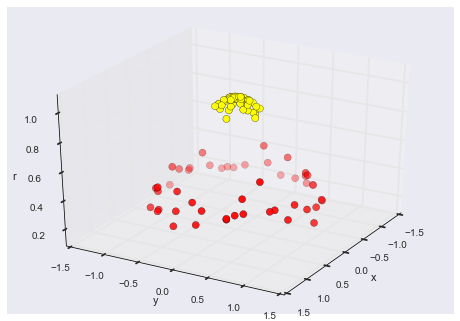
\includegraphics[width=0.9\linewidth]{Immagini/SVM kernel.png}
		\captionsetup{width=.8\linewidth}
		\caption{Punti scalati mantenendo uguali le coordinate x e y e
			calcolando z secondo $e^{-(x^2 + y^2)} + 1$ \cite{Data science handbook}}
	\end{subfigure}

	
\end{figure}

Spesso però i dati reali non sono cosi nettamente separabili e avremmo una zona
in cui dati di diverse categorie si sovrappongono. Per gestire al meglio questi
casi il modello ha un iperparametro $C$ che consente di specificare il grado di
rigidità del margine: con una $C$ molto grande avremmo una separazione molto
netta in cui nessun punto si trova all'interno del margine, al contrario con
una $C$ piccola permettiamo al modello di includere dei punti nel margine. $C$ è
utile anche per evitare che il nostro vettore sia troppo influenzato dalla
presenza di outlier: con un margine rigido l'iperpiano dovrà essere tracciato
massimizzando la sua distanza dall'outlier mentre ammettendo che questo ricada
all'interno del margine potremmo tracciare un iperpiano che massimizzi la distanza dai
dati reali.


\section{Alberi di decisione e foreste casuali}

L'obbiettivo è costruire un albero di decisione ovvero un albero in cui a ogni
nodo in base al valore di una caratteristica del dato il processo di
classificazione procede lungo uno dei sotto alberi fino a arrivare a una foglia
che stabilisce la categoria del dato.

Ogni decisione consiste quindi nel confrontare una caratteristica con un valore
di soglia ed è quindi necessario scegliere un valore che al meglio separi i dati
nelle corrette categorie. Per fare questo ci serviamo di un indice di
eterogeneità statistica, come l'indice di Gini o l'entropia, scegliendo il
valore della soglia che massimizza l'eterogeneità media delle categorie dei due
sottoinsiemi di dati prodotti dalla decisione ovvero due gruppi tali che ognuno
è il più vicino possibile a avere una sola categoria di dati.

Un problema di questo approccio è che tende a fare overfitting ovvero creare un
albero troppo adattato ai dati di training che poi non classifica correttamente
i dati reali soprattutto aumentando troppo la profondità dell'albero. Per
risolvere questo problema possiamo modificare i valori degli iperparametri come
la profondità massima o il numero minimo di dati per foglia oppure possiamo
usare un'altra tecnica: le foreste casuali. Le foreste casuali sono un
classificatore che aggrega una serie di alberi di decisioni prendendo la
classificazione più popolare tra questi. Per realizzarlo vengono allenati più
alberi di decisione con diversi sottoinsiemi dei dati di training e la
classificazione finale sarà ottenuta prendendo la classificazione più frequente
tra i diversi alberi di decisione.

\section{Naive Bayes}

Naive Bayes si basa sull'applicazione del teorema di Bayes:
$$
P(Y=y \mid X_1=x_1, \dots, X_n=x_n \mid Y=y) = \frac{P(Y=y) P(X_1=x_1, \dots, X_n=x_n \mid Y=y)}
                                 						{P(X_1=x_1, \dots, X_n=x_n)}
$$

dove $Y = y$ è l'evento che si verifica quando la categoria da predire è $y$ e
per $i = 1, ..., n$, $X_i = x_i$ è l'evento che si verifica quando la i-esima
caratteristica del dato da classificare assume il valore $x_i$. 

% Una delle
% ipotesi del teorema è  che le variabili $X_i \dots X_n$ siano tra loro indipendenti, questo non è
% sempre vero ma in problemi reali si può tipicamente assumerlo come vero e
% ottenere comunque buoni risultati.

Possiamo stimare $P(y)$, $P(X_1 = x_1 \mid y), \dots, P(X_n = x_n \mid Y)$ e $P(x_1, \dots, x_n)$
dalle frequenze del training set e quindi calcolare la probabilità che un dato
appartenga a una categoria. Fatto questo basterà assegnargli la categoria a cui è
più probabile che appartenga.

Questo approccio si basa su due importanti assunzioni: la prima è che le
variabili $X_i \dots X_n$ siano tra loro indipendenti, la seconda che la
frequenza delle probabilità nel training set sia sufficientemente precisa nello
stimare le probabilità reali. Seppure non abbiamo prova di queste assunzioni
spesso con dati reali riusciamo a ottenere un buon stimatore anche se le ipotesi
non sono del tutto vere.

\section{K-means}

K-means è l'unico algoritmo non supervisionato usato in questo progetto e si
basa sul dividere il training set in K categorie scegliendo K punti detti
baricentri e assegnando ogni dato alla categoria del baricentro più vicino. La
posizione dei baricentri viene ottimizzata cercando di minimizzare la somma
delle distanze quadratiche tra i dati del training set e il loro baricentro più
vicino.
$$
\sum_{i=0}^{n}\min_{\mu_j \in C}(||x_i - \mu_j||^2),
$$

dove $n$ è il numero di dati di training, $C$ è l'insieme dei baricentri,
$\mu_j$ è quindi il j-esimo baricentro e $x_i$ è l'i-esimo dato.

Essendo questo un algoritmo non supervisionato non è nota l'associazione tra
baricentro e categoria reale e sarà quindi necessario ristabilire questa
associazione ad esempio associando ogni baricentro alla categoria più presente
nel suo insieme. Questa associazione non sarà sempre uno a uno infatti potrebbe
essere vantaggioso avere più baricentri che categorie reali associando più
baricentri alla stessa categoria.


% 
% 
%			CAPITOLO 2: Il problema affrontato
\chapter{Il problema affrontato}
\label{cap2}
\section{Descrizione dei dati}
I dati consistono in una serie di misurazioni fatte su dei reperti archeologici,
le misurazioni consentono di sapere la composizione dei materiali 

\section{Ambiente software}
Python 3.7
scikit-learn==0.21.3
numpy==1.16.5
pandas==0.25.1

\section{Schema delle prove}


\subsection{Repeated hold out}
Per hold out si intende la tecnica di valutazione di un algoritmo basata sul
separare i dati disponibili in un insieme di training e uno di testing. Il primo
insieme verrà usato per allenare il modello, il secondo per valutarlo.
Nonostante questo porti ad allenare il modello con meno dati 

\subsection{Convalida incrociata}


\subsection{Griglia di ricerca}



% 
% 
%			CAPITOLO 3: Risultati
\chapter{Risultati}
\label{cap3}
\section{Valutazione combinata}

% 
% 
%			CAPITOLO 4: Conclusioni
\chapter{Conclusioni}
\label{cap4}

%
%			BIBLIOGRAFIA
%
\begin{thebibliography}{00}
%
% \bibitem{gotti91}
% M. Gotti, I linguaggi specialistici, Firenze, La Nuova Italia, 1991.
%
\bibitem{Intro to nn}
D. Kriesel, A brief introduction to neural networks, available at
http://www.dkriesel.com, 2007. %Seguendo "how to cite" sul sito
%

% https://towardsdatascience.com/support-vector-machine-introduction-to-machine-learning-algorithms-934a444fca47
\bibitem{Data science handbook}
Jake VanderPlas, Python Data Science Handbook, O'Reilly Media, aviable at
https://jakevdp.github.io/PythonDataScienceHandbook/, 2016

\bibitem{scikit} %TODO: fare bene la citazione
https://scikit-learn.org


\end{thebibliography}
% 
\end{document}


 
